\section{Implementation}

In this section the author discusses the implementation of the experimental system to prove the concept of our proposed load balancers with ECMP redundancy in detail.

\subsection{Experimental system architecture}\label{sec:poc}

\begin{figure}[tb]
\begin{center}
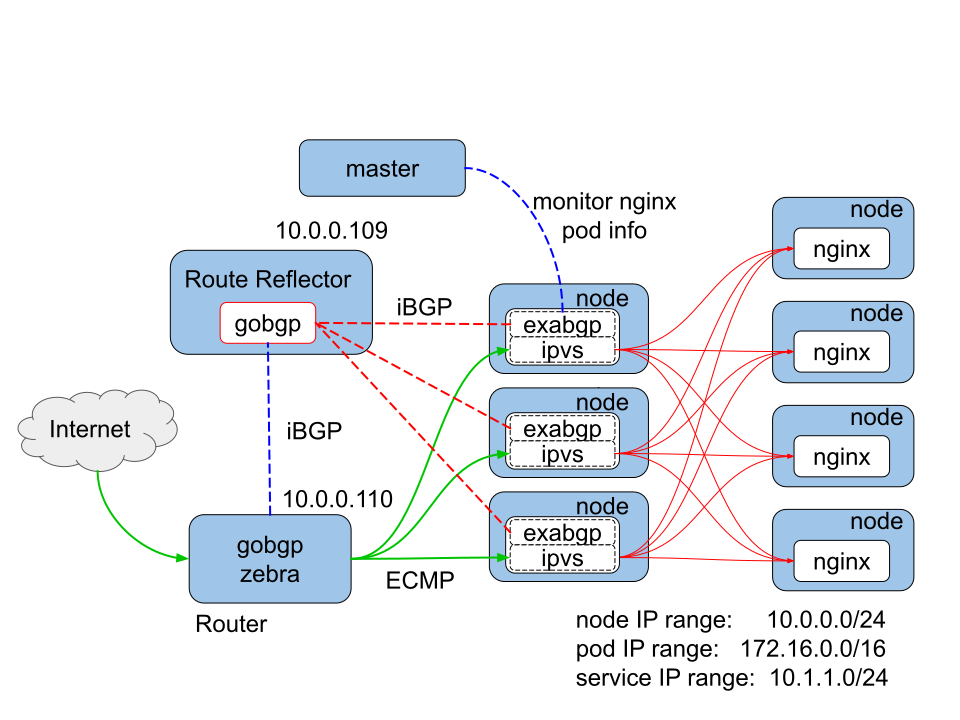
\includegraphics[width=0.8\columnwidth]{Figs/poc.png}
\end{center}
\caption{An experimental container cluster with proposed redundant software balancers}
\centering\parbox[c]{0.9\columnwidth}{
  The master and nodes are configured as Kubernetes's master and nodes on top of conventional Linux boxes, respectively.
  The route reflector and the upstream router are also conventional Linux boxes.
  For the green lines, a service IP address is used. The red lines use the IP addresses of the overlay network. The blue line uses the IP addresses of the node network.
}

\label{fig:poc}
\end{figure}

Fig.~\ref{fig:poc} shows the schematic diagram of proof of concept container cluster system with the proposed software load balancers.
%
Each load balancer pod consists of an exabgp container and an ipvs container.
The ipvs container is responsible for distributing the traffic toward the service IP to web server(nginx) pods.
The IP address for nginx pods and load balancer pods are dynamically assigned upon launch of themselves from 172.16.0.0/16 address range.
The ipvs container monitors the availability of web server pods by consulting apiserver on the master node and manages the load balancing rule appropriately.
The exabgp container is responsible for advertising the route toward the service IP to the route reflector.
The route reflector aggregates the routing information advertised by load balancer pods and advertise them to the upstream router.
The upstream router updates its routing table according to the advertisement.

All the nodes and route reflector are configured using Debian 9.5 with self compiled linux-4.16.12 kernel.  
The author also used conventional Linux box as an upstream router for testing purpose, using the same OS as the nodes and route reflector.
The version of Linux kernel needed to be 4.12 or later to support hash based ECMP routing table.
The author also needed to enable kernel config option CONFIG\_IP\_ROUTE\_MULTIPATH\cite{ipsysctl} when compiling, and set the kernel parameter fib\_multipath\_hash\_policy=1 at run time.
Although in the actual production environment, proprietary hardware router with the highest throughput is usually deployed, one can still test some of the advanced features by using a Linux box as the router.

\begin{table}[H]
  \centering
  \begin{tabular}{|l|c|c|c|}
    \hline
    & \multicolumn{1}{c|}{gobgp} & \multicolumn{1}{c|}{exabgp} & \multicolumn{1}{c|}{bird} \\ \hline
    \begin{tabular}{l} Static route advertisement\\ without injector$^{*}$ \end{tabular} & No  & Yes & No \\ \hline
    \begin{tabular}{l} add-path support$^{**}$ \end{tabular} & Yes & No & Yes  \\ \hline
    \begin{tabular}{l} FIB manupilation \end{tabular} & Yes(through zebra) & No & Yes(Native) \\ \hline
    \begin{tabular}{l} Use case \end{tabular} & Router/Route reflector & Load balancer & Not used$^{***}$  \\ \hline
  \end{tabular}
  \caption{Comparison of open source BGP agents}
  \centering\parbox[c]{0.9\columnwidth}{
    Open source BGP agents are compared in terms of the features required in the proposed systems. \par
    \small
    $^{*}$ \phantom{$^{**}$} The injector is a program that injects static route, other than the BGP daemon itself. \par
    $^{**}$ \phantom{$^{*}$} The add-path is the feature to support multipath advertisement. \par
    $^{***}$ \phantom{$^{}$} Configuration of bird was more omplex than other agents.
  }
  \label{table:bgp_agents}
\end{table}

Table~\ref{table:bgp_agents} compares open source BGP agents in terms of required features for the proposed architecture.
Each load balancer {\em pod} needs to advertise a static route for the service IP to itself. 
For that purpose, exabgp is preferable due to its simplicity.
As for the route reflector, add-path\cite{rfc7911} feature is needed for multi-path advertisement, which is supported by gobgp.
For the upstream router Forwarding Information Base(FIB) manipulation\cite{exa-networks_2018} feature is needed, which is supported by gobgp.
As a result, exabgp is used for the load balancer pods, and gobgp is used for the route reflector and the upstream router.

The other features needed for the route reflector are a dynamic-neighbor feature to describe peer group as a range of IP address, and overlay network feature on the Linux box.
The configurations for the upstream router is summarised in \ref{appendix:router_config}.
The configurations for the route reflector is summarised in \ref{appendix:route_reflector_config}.

\subsection{Ipvs container}\label{sec:ipvs}

The proposed load balancer needs to dynamically reconfigure the ipvs balancing rules whenever {\em pods} are created or deleted. 
Fig.~\ref{fig:ipvs-ingress-schem} is a schematic diagram of ipvs container to show the dynamic reconfiguration of the ipvs rules.
Two daemon programs, controller and keepalived, running in the container are illustrated.
The keepalived manages Linux kernel's ipvs rules depending on the ipvs.conf configuration file.
It can also periodically health check the liveness of a {\em real server}, 
which is represented as a combination of the IP addresses and port numbers of the target {\em pods}. 
If the health check to a {\em real server} fails, keepalived will remove that {\em real server} from the ipvs rules immediately.
The interval of the health check is typically 1 to several seconds and is arbitrarily determined by users.  

\begin{figure}[h]
  \begin{center}
    \includegraphics[width=0.8\columnwidth]{Figs/ipvs-ingress-schem}
    \caption{Implementation of ipvs container.}
    \label{fig:IPVS-ingress-schem}

    \parbox[c]{0.9\columnwidth}{
      The controller checks the pod status every second, by consulting the master node.
      Upon a change of the status, the controller updates the ipvs.conf and sends SIGHUP to keepalived.
      The keepalived reload the ipvs.conf and updates the load balancing rules in the kernel correctly.
    }
  \end{center}

\end{figure}

Every second, the controller monitors information concerning the running {\em pods} of a web application in the Kubernetes cluster by consulting the apiserver running in the master through its API.
Whenever {\em pods} are created or deleted, the controller notices the change and automatically regenerate an appropriate ipvs.conf 
and issue SIGHUP to keepalived within a second.
Then, keepalived will reload the ipvs.conf, and modify the kernel's ipvs rules correctly depending on the result of the health check.

When a pod is terminated, existing connections are reset by the node kernel.
The SYN packets sent to a pod after termination, but before the ipvs rule update, will be answered with ICMP unreachable by the node.
In these cases, the client sees connection errors.
In order to avoid the connection errors to be seen by a human, HTTP client programs are required to re-initiate the connection.
However, since the load balancer rule update is within a second, these errors can be regarded as the tolerable rare exceptions even without such re-initiations.

The actual controller\cite{ktaka_ccmp_2017_826894} is implemented using the Kubernetes ingress controller\cite{K8sIngress2017} framework. 
By importing existing Golang package, \enquote{k8s.io/ingress/core/pkg/ingress}, the author could simplify the implementation, e.g. 
120 lines of code.  
%
Keepalived and the controller are placed in the docker image of ipvs container.
The ipvs is the kernel function and namespace separation for container has already been supported in the recent Linux kernel. 

Configurations for capabilities were needed when deploying the ipvs container: adding the CAP\_SYS\_MODULE capability 
to the container to allow the kernel to load required kernel modules inside a container, 
and adding CAP\_NET\_ADMIN capability to the container to allow keepalived to manipulate the kernel's ipvs rules. 
For the former case, the author also needed to mount the \enquote{/lib/module} of the node's file system on the container's file system.

\begin{figure}[h]
  \centering
  \begin{minipage}{0.7\columnwidth}
    \begin{lstlisting}[frame=single]
      virtual_server fwmark 1 {
        delay_loop 5
        lb_algo lc
        lb_kind NAT
        protocol TCP
        real_server 172.16.21.2 80 {
          uthreshold 20000
          TCP_CHECK {
            connect_timeout 5
        connect_port 80
          }
        }
        real_server 172.16.80.2 80 {
          uthreshold 20000
          TCP_CHECK {
            connect_timeout 5
            connect_port 80
          }
        }
      }
    \end{lstlisting}
  \end{minipage}

  \caption{An example of ipvs.conf}
  \label{fig:ipvs.conf}

  \begin{minipage}{0.9\columnwidth}
    This configuration file is auto-generated by the controller.
    The controller periodically accesses the apiserver on the master node and constantly monitor the status of running pods.
  \end{minipage}
\end{figure}

\begin{figure}[h]
  \centering
  \rule{\columnwidth}{0.4pt}
\begin{verbatim}
# kubectl exec -it IPVS-controller-4117154712-kv633 -- IPVSadm -L
IP Virtual Server version 1.2.1 (size=4096)
Prot LocalAddress:Port Scheduler Flags
  -> RemoteAddress:Port Forward Weight ActiveConn InActConn
FWM  1 lc
  -> 172.16.21.2:80      Masq    1      0          0         
  -> 172.16.80.2:80      Masq    1      0          0
\end{verbatim}
\rule{\columnwidth}{0.4pt}

\caption{Example of IPVS balancing rules}
\label{fig:IPVS rule}

\begin{minipage}{0.9\columnwidth}
  This shows the load balancing rule in a load balancer container.
  The packet that has FWM(fwmark)=1 will be forwarded to two real servers using the least connection(lc) balancing algorithm.
  The fwmark is a parameter that is only available inside a socket buffer in Linux kernel.
  The fwmark can be put and manipulated by the iptables program, once a socket buffer for a received packet is assigned by the kernel.
\end{minipage}
\end{figure}

Figure~\ref{fig:ipvs.conf} and Figure~\ref{fig:IPVS rule} show an example of an ipvs.conf file 
generated by the controller and the corresponding IPVS load balancing rules, respectively.
Here, we can see that the packet with {\tt fwmark=1}\cite{BertHubert2002} is distributed 
to {\tt 172.16.21.2:80} and {\tt 172.16.80.2:80} 
using the masquerade mode(Masq) and 
the least connection(lc)\cite{Zhang2000} balancing algorithm.

\subsection{BGP software container}\label{sec:bgp}

\begin{figure}[tb]
  \begin{center}
    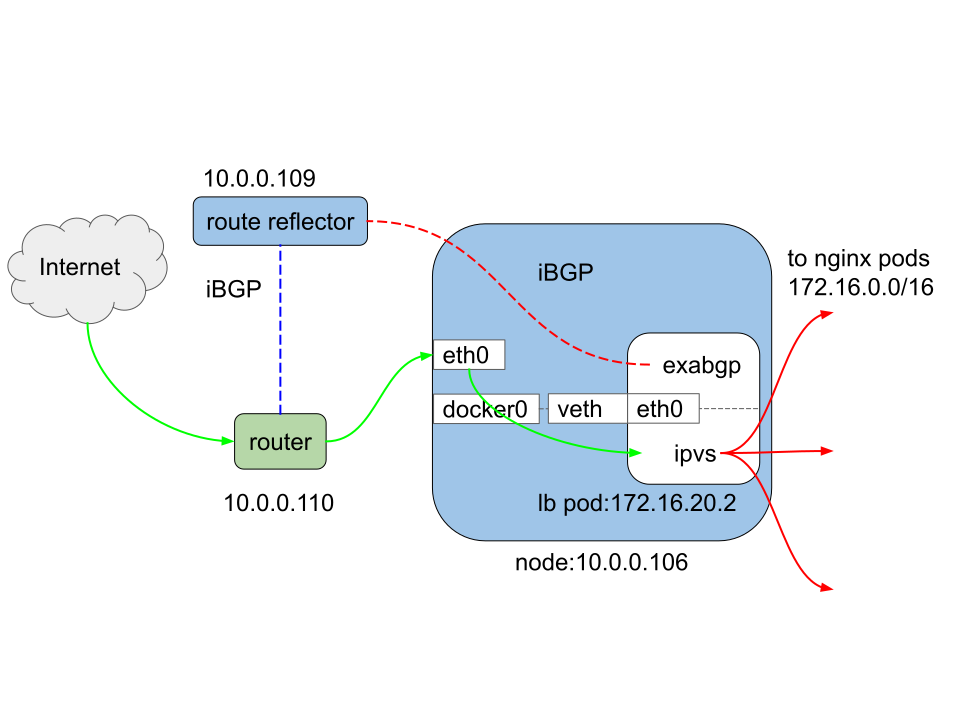
\includegraphics[width=0.8\columnwidth]{Figs/exabgp}
    \caption{Network path by the exabgp container}
    \label{fig:exabgp_schem}
  
    \parbox[c]{0.9\columnwidth}{
      The packets from Internet to service IPs, 10.1.1.0/24 are routed to the load balancer pod(green arrows) by the set of routing rules shown in Table~\ref{table:exabgp_setting}.
      And then the ipvs container forwards them to nginx pods(red arrows).
      The IP address of any pod is dynamically assigned from 172.16.0.0/16 when the pod is started. 
    }
  \end{center}
\end{figure}

\begin{table}
  \begin{center}
    \begin{tabular}{lllr}
      \hline 
      \multicolumn{4}{l}{[BGP announcement]} \\
      \hspace{15 mm} & \multicolumn{2}{l}{route 10.1.1.0/24 next-hop 10.0.0.106} & ...(1) \\
      \multicolumn{4}{l}{[Routing in node net namespace]} \\
      \hspace{15 mm} & \multicolumn{2}{l}{ip netns exec node ip route replace 10.1.1.0/24 dev docker0} & ...(2) \\
      \multicolumn{4}{l}{[Accept as local]} \\
      \hspace{15 mm} & \multicolumn{2}{l}{ip route add local 10.1.1.0/24 dev eth0} & ...(3) \\
      \hline
    \end{tabular}
    \caption{Required settings in the exabgp container}
    \label{table:exabgp_setting}
  
    \parbox[c]{0.9\columnwidth}{
      (1) The node IP address, 10.0.0.106 is used as next-hop for the service IPs, 10.1.1.0/24, in BGP announcement.
      (2) In order to route the packets destined toward the service IP to the container, a routing rule to the dev docker0 is created in the node net namespace. 
      (3) A routing rule to accept the packets destined toward the service IPs,  as local is also required.
    }
  \end{center}
\end{table}

In order to implement the ECMP redundancy, the author also containerized exabgp using Docker.
Figure~\ref{fig:exabgp_schem} shows a schematic diagram of the network path realized by the exabgp container.
As mentioned earlier, the author used exabgp as the BGP advertiser. 
The ingress traffic from the Internet is forwarded by ECMP routing table on the router to the node that hosts a load balancer pod.
And then it is routed to the load balancer pod according to the set of routing rules in Figure~\ref{fig:exabgp_schem}.
After that the ipvs forwards them to nginx pods.
The IP address of any pod is dynamically assigned from 172.16.0.0/16 when the pod is started. 

Table~\ref{table:exabgp_setting} summarises some key settings required in the exabgp container to route the traffic to the ipvs container.
In BGP announcements the node IP address, 10.0.0.106 is used as the next-hop for the service IPs, 10.1.1.0/24.
Then on the node, in order to route the packets toward the service IPs to the ipvs container, 
a routing rule for 10.1.1.0/24 to the dev docker0 is created in the node net namespace. 
A routing rule to accept the packets toward the service IPs as local is also required in the container net namespace. 
A configuration for exabgp is shown in \ref{appendix:exabgp_config}.

\FloatBarrier

\mytodo[inline]{Add a mention about ingress controller implementation, if possible.}


\section{Summary}
In this chapter the author provided discussion of load balancer architecture and its implementations suitable for container clusters.

First the author discussed problems of conventional architecture. 
Since Kubernetes is dependent on external load balancers provided by the cloud infrastructures, 
it failed to provide portability of a web application in environments where there was no supported load balancer. 
Furthermore the routes ingress traffic from the internet follow were very complex and inefficient.

In order to alleviate these problems, the author proposed a cluster of software load balancers in containers.
The proposed load balancers utilized container technotlogy and was managed by Kubernetes.
As a result, it is runnable on any environment including cloud infrastructures and on-premise data centes.
Furthermore, since Kubernetes manages load balancer containers, it can quickly scale the number containers depending on the demand.

The author also discussed redundant architecture using ECMP with BGP for proposed load balancer containers.
By using the ECMP, the upstream router can route the ingress traffic to a cluster of load balancer containers in a redundant and scalable mannar.
By using BGP, which is the standard protocol, ECMP routing rules in the upstream router are automatically populated, upon the launch of load balancer containers.

As a result users, i.e., web application providers can quickly and automatically set up routes to their web application, upon its launch.
This will greatly improve the portability of a web application and there by enables migrations.


